%!TEX encoding = UTF-8 Unicode
\subsection{Fog Computing Architecture}
\label{sec:fog_architecture}
\noindent Fog computing is a great resource to support IoT applications' requirements in mobile environments. Taking into account what has been mentioned in Section \ref{sec:Introduction} and Section \ref{sec:Computingparadigms}, it has the following fundamental characteristics which validate the statement uttered above (refer to Table \ref{computing_paradigms}):
\begin{itemize}
	\item \textbf{Heterogeneity support}. Supports collection and processing of data of different actors acquired through multiple types of network communication, wide diversity applications and services;
	\item \textbf{Geographical distribution}. Uses anything between the cloud and \textit{things} to provide ubiquitous computing, allowing continuity of service in mobile environments;
	\item \textbf{Contextual location awareness, and low latency}. Provides low latency due to the proximity between the IoT devices and the fog nodes. Also, the contextual location allows them to be aware of the cost of communication latency with both other fog nodes and the end devices, allowing the distribution of applications across the network to be organized in a weighted manner;
	\item \textbf{Mobility support}. The exponential growth of mobile devices demands support for mobility techniques;
	\item \textbf{Real-time interactions}. Applications may involve real-time interactions rather than batch processing (e.g., as cloud does);
	\item \textbf{Scalability and agility of federated, fog-node clusters}. Fog is adaptive; may form clusters-of-nodes or cluster-of-clusters to support elastic compute, resource pooling, etc., supporting large-scale applications;
	\item \textbf{Multiple IoT applications}. Fog devices handle multiple IoT applications competing for their limited resources;
	\item \textbf{Virtualization support}. Introduces a software abstraction between the hardware and the OS and application running on the hardware;
	\item \textbf{Interoperability and federation}. Uses cooperation of different providers to support heavy applications such as real-time streaming. Moreover, it supports migration of applications to more suited fog servers depending on the current context;
	\item \textbf{Predominance of wireless access}. Most of the end devices only support wireless communication.
\end{itemize}

Nonetheless, as stated in Section \ref{subsec:Objectives}, fog still has some limitations. In order to tackle those, its overall architecture must be understood. This includes knowing: what are the actors and how they interact, how IoT nodes connect to the fog servers, how clients outsource the allocation and management of resources that they rely upon to these servers, how migration is performed, etc.

\subsubsection{Actors}
\noindent\tab Figure \ref{fog_architecture} shows the typical fog computing architecture. As stated before, mist computing can be implemented in a layer between the fog servers and the end devices. Moreover, the presence of cloud servers is not imperative however, it is very important for numerous applications.

\begin{figure}[t]
	\centering
	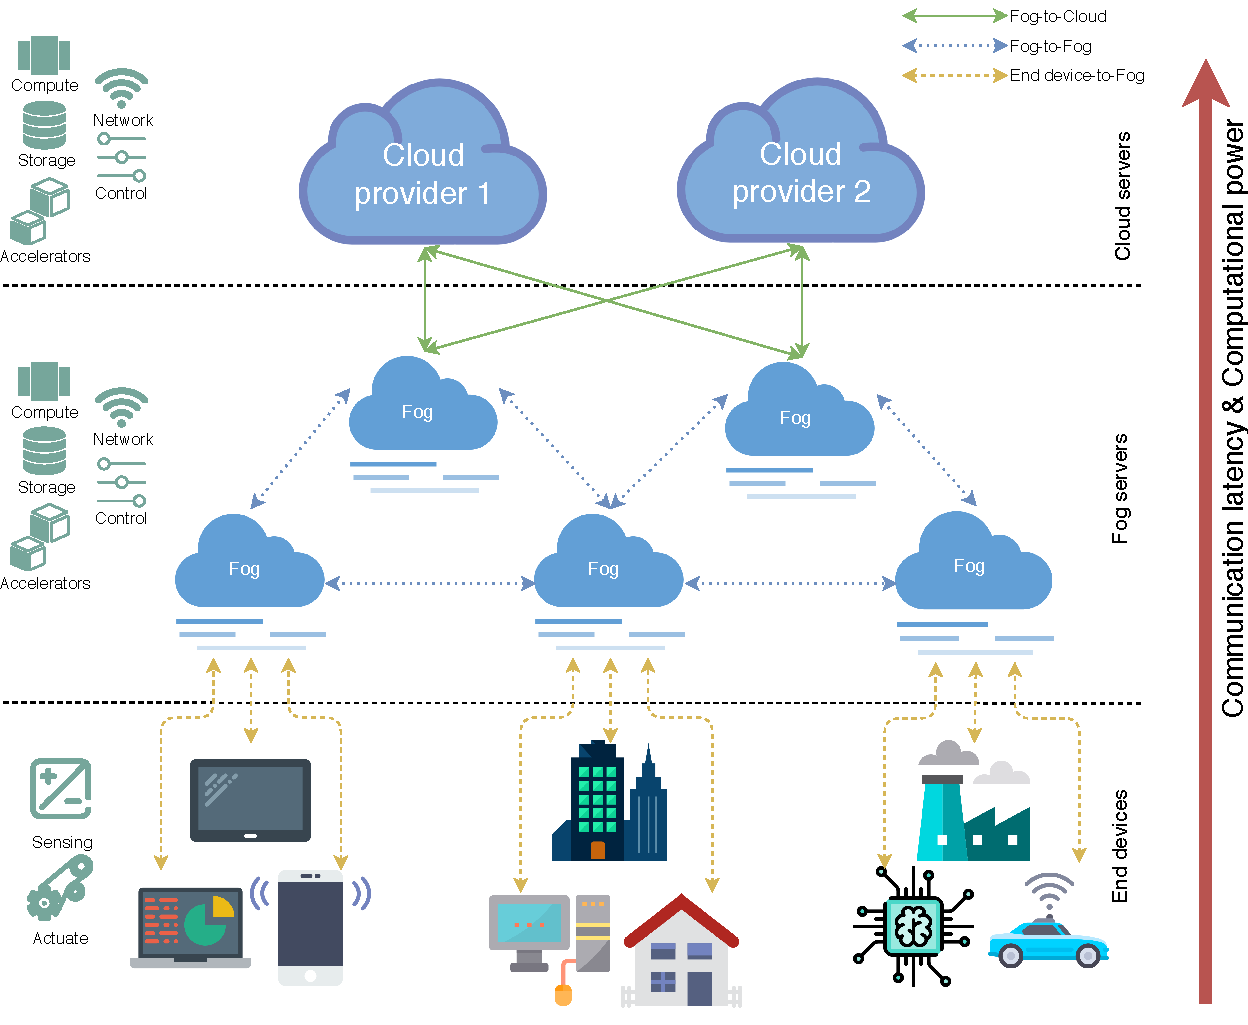
\includegraphics[width=0.9\textwidth]{images/fog_architecture/fog_architecture}
	\caption{Typical architecture of fog computing.}
	\label{fog_architecture}
\end{figure}

\noindent\tab Fog computing layer is composed by fog nodes/servers, which allow the deployment of distributed, latency-aware applications and services. Those nodes can be either physical (e.g., gateways, switches, routers, servers) or virtual (e.g., virtualized switches, virtual machines, cloudlets) components which provide computing resources to the connected end devices. When needed, they also provide network connectivity to centralized services (i.e. cloud). Moreover, fog nodes can operate in a centralized or decentralized manner or even be configured as stand-alone nodes. Therefore, they are the fundamental components in this three tier architecture (i.e. IoT-fog-cloud), being able to support the six features shown below \cite{iorga2018fog}:
\begin{itemize}
	\item \textbf{Autonomy}. Fog nodes can be autonomous enough to operate independently, making local decisions, at the node or cluster-of-nodes level;
	\item \textbf{Heterogeneity}. Can be deployed in a wide variety of environments;
	\item \textbf{Hierarchical clustering}. Fog network can be organized with an arbitrary number of layers, being able to provide different subsets of service functions while working together as a continuum;
	\item \textbf{Manageability}. They are managed and orchestrated by complex systems that can perform most routine operations automatically;
	\item \textbf{Programmability}. Fog nodes are inherently programmable at multiple levels, by multiple stakeholders such as network operators, domain experts, equipment providers, or end users.
\end{itemize}

\noindent\tab Fog nodes are of most value in scenarios where data needs to be collected at the edge and where data from thousands or even millions of devices is analyzed and acted upon in micro and milliseconds \cite{openfog2017openfog}. In order to being able to support such large number of requests, especially those engaged in enhanced analytics, fog nodes may implement additional hardware. Accelerators modules (refer to Fig. \ref{fog_architecture}) can be implemented to provide supplementary computational throughput. For instance, hardware accelerators can be performed through Graphics Processing Units (GPUs); they are an optimal choice for applications that support parallelism or for stream processing. Also, fog nodes may be equipped with Field Programmable Gate Arrays (FPGAs) or even Digital Signal Processors (DSPs) for this propose.\\
\noindent\tab It is worth noting that, once fog nodes can be anything with computational and storage power in the cloud-to-things continuum, the links formed in these architectures (i.e. End device-to-Fog, Fog-to-Fog and Fog-to-Cloud) can be of any type. For instance, end devices can be connected to fog servers by wireless access technologies (e.g., WLAN, WiFi, 3G, 4G, ZigBee, Bluetooth) or wired connection. Moreover, fog nodes can be interconnected by wired or wireless communication technologies, and they can be linked into the cloud by core network using fiber transmission with low-latency.\\
\noindent\tab In this architecture, the connected sensors located at the edge, generate data that can adopt two models. First, in a sense-process-actuate model, the information collected is transmitted as data streams, which is acted upon by applications running on fog devices and the resultant commands are sent to actuators. In this model, the raw data collected often does not need to be transferred to the cloud; data can be processed, filtered, or aggregated in fog nodes, producing reduced data sets. The result can then be either stored inside fog nodes or actuated upon through the actuators. Second, in a stream-processing model, sensors also send data streams, where the information mined (from the incoming streams) is stored in data centers for large-scale and long-term analytics. In this case, big data needs to be stored and does not have significant latency constraints. Being fog servers less powerful than the cloud ones, cloud is far more suited for this kind of operations. Yet, fog servers can still shrink data, doing some intermediate processing as in the previous model. This meets the aforementioned statement - although cloud is not always essential for the functioning of fog, in some applications it is beneficial or even crucial.\\
\noindent\tab The applications deployed by the connected end users into the fog nodes can be treated either as a whole or as a Distributed Data Flow (DDF) programming model, in which the applications are moduled as a collection of modules. DDF is proposed by N. Giang et al. \cite{giang2015developing} for IoT applications that utilize computing infrastructures across the fog and the cloud, allowing the application flow to be deployed on multiple physical devices rather than one. This can be particular useful to deploy less restricted modules in terms of latency to the upper fog layers (ideally to the cloud), leaving the fog nodes in the lower layers less overloaded, being able to respond faster to modules within tighter latency bounds. As already mentioned, fog utilizes virtualization mechanisms due to the numerous advantages offered. Hence, hosting an application involves creating a set of VMs or execution containers (e.g., Docker) and assign them to a set of physical or virtual components along the cloud-to-things continuum.

\subsubsection{Orchestration}\label{sec:fog_arch_orchestration}
\noindent\tab When an end device needs to offload some work to a third party, it needs somehow to know where to outsource the allocation and management of resources. To do so, this architecture also needs a discovery service which concerns in finding the best available fog server, given certain capabilities and requirements. In this context, J. Gedeon et al. \cite{gedeon2017router}, propose a brokering mechanism in which available surrogates (i.e. fog nodes) advertise themselves to the broker. When it receives client requests, considering a number of attributes such as network information, hardware capabilities, and distance, it finds the best available surrogate for the client.\\
%This mechanism can be implemented on standard home routers, and thus, leverages the ubiquity of such devices in urban environments. Multiple brokers are interconnected using Distributed Hash Tables (DHTs) in order to exchange information.\\
%OK
\noindent\tab Finally, fog also needs an orchestration layer in order to monitor the current context to be able to take management decisions with regard to applications and data placement. In this context, C. Guerrero et al. \cite{guerrero2018influence} state that most of the literature considers the existence of a central broker or orchestrator gathering all system information (i.e. monitoring fog devices, clients, cloud and services), leading to poor scalability and high orchestration algorithm complexity when the number of elements is high (e.g., in smart cities). To overcome this bottleneck, O. Skarlat et al. \cite{skarlat2016resource,skarlat2017optimized} consider the concept of fog colonies. Each colony has an orchestrator and an arbitrary number of fog cells (a software component running on fog nodes). These fog cells are responsible for receiving tasks from IoT devices, and depending on the available resources, decide whether to execute it in the current fog node or to transfer it to the orchestrator. This top hierarchic element (inside a colony) will then migrate this task to the cloud or to another fog colony, if the current one is not able to handle it. The authors also state that these orchestrators could be replaced applying a decentralized approach. However, it would lead to extensive coordination and voting between the involved fog cells. On the other hand, F. Bonomi et al. \cite{bonomi2014fog} propose a distributed orchestration. This is performed implementing a Foglet software agent in each fog node. It has small footprint yet capable of monitoring machine's health and state. This information is then pushed to the distributed and persistent storage for global processing. The distributed database is also responsible for storing business policies defined by the fog administrators. The distributed policy is then embedded in every Foglet. Specifically, when a Foglet receives a request, it will gather policies from the policy repository and information relative to the currently active service instances from the services directory. With these informations, it tries to find an instance that satisfies the defined constraints. If such was found it, forwards the request, otherwise a new instance needs to be created.\\
%OK
\noindent\tab Upon the decision to migrate some application/module, service continuity is an important parameter once downtime may degrade the perceived QoS by the end user. To perform this operation, the exploited technologies are the VMs and containers. For instance, VM synthesis reduces the image size by splitting it into multiple layers, transferring only the application-specific layer which includes both the static binary program and the runtime memory data \cite{ma2017efficient}. However, this can still involve hundreds of megabytes. Also, live migration was introduced to reduce the downtime from the traditional non-live migration. The latter, suspends the VM, transfers all the content from one physical machine to another and resumes it only after the process, continuing from the same state as before suspension. On the other hand, to perform live migration there are two different approaches. The pre-copy memory migration firstly transfers VM’s memory state. Meanwhile, the VM keeps running. If a page gets modified (dirtied), it will be re-sent. This keeps going until either a small, Writable Working Set (WWS) has been identified, or a given number of iterations is reached. Then, the VM is suspended and sent along with the remaining dirtied pages to the target machine. On the other hand, post-copy creates and sends a snapshot of the VM state from the source physical machine to the destination, being launched at its completion. Meanwhile, during the transfer, the VM is still running in the source machine. Upon copy completion, the memory state that was kept changing is copied on demand (by page-faults) from the source to the destination machine, reducing the downtime service and (avoiding) denial of services to the end devices \cite{hines2009post}.\\
%OK
\noindent\tab Despite these advances, this process can be impractical in mobile fog environments due to its large size. Container represents a lighter virtualization technique. It allows developers to package up an application with all the parts needed (e.g., libraries and other dependencies). These applications share the OS of the physical machine and some libraries and/or binaries, allowing container's size to be much smaller. This eases both the migration and hosting applications (i.e. more applications in a single machine and does not require restarting the OS upon migration) \cite{saurez2016incremental}.\\
%OK
\noindent\tab Nonetheless, there are two different approaches that can be exploited and implemented into the migration decisions. On the one hand, the reactive approach, as the name suggests, only performs migration when it is needed. When users and fog nodes become out of range, migration is performed to ensure QoS in mobile environments. However, I. Farris et al. \cite{farris2017optimizing} argue that downtime is not the only degrading factor of service continuity, but also the overall migration which impacts user's Quality of Experience (QoE). This way, on the other hand, exists the proactive approach that deploys replicas of the user service in neighboring fog nodes (e.g., using mobility patterns). Also, periodically the state in these nodes is updated. The main goal is to reduce the migration time and improve users' QoE. However, this brings new costs at different levels such as computation, memory, and networking.\\
%For this propose, E. Saurez et al. \cite{saurez2016incremental} propose foglets, a programming model that facilitates distributed programming across fog nodes. It is implemented through container-based visualization. Foglets not only provides APIs for application development as DDFs, including the primitives for communication between the application components, but also embodies algorithms for the discovery and incremental deployment of resources commensurate with the application needs. Moreover it provides mechanisms for QoS-sensitive and workload sensitive migration of application components due to end devices mobility and application dynamism. Specifically, there are four entities in the foglets runtime system: the discovery server, the docker registry server, the entry point daemon, and the worker process. The discovery server is a partitioned name server that maintains a list of fog nodes available. Docker registry server is a server that contains the binaries for the applications that have been launched on the foglets infrastructure. The entry point daemon executes directly on top of the host OS in the fog node, awaits requests and periodically sends ``I am alive'' message to the discovery server. Finally the worker process carries out the functionality contained in a particular application component assigned to it.\\
\noindent\tab Fog servers can provide reduced latencies and help in avoiding/reducing traffic congestion in the network core. However, this comes at a price: more complex and sophisticated resource management mechanisms are needed. This raises new challenges to be overcome such as dynamically deciding when, and where (device/fog/cloud) to carry out processing of requests to meet their QoS requirements. Furthermore, in mobile environments such mechanisms must incorporate mobility (i.e. location) of data sources, sinks and fog servers in the resource management and allocation process policies to promote and take advantage of proximity between fog and end devices.